Because using more superdiagonals did not improve the preconditioner, we will go in the other direction by using both the super- and subdiagonals. We will test using \(\left\lbrace 1,2,3,4\right\rbrace\) super- and subdiagonals with 1 partition in each diagonal, leading to \(\left\lbrace 2,4,6,8\right\rbrace\) different coefficients that needs to be learned. 

Immediately from the learning curves in figure \ref{fig: super sub learning curves} seed 0, we see a sizeable improvement. With the plateaued mean solver iteration count around 1750 and median around 1500, compared with the runs of previous section \ref{sec: num super} having plateaued around mean of 2100 and median of 1800 solver iteration count. Because of the large improvement, the test was run again with a different seed to ensure improvement was not because of the seed of the data set and start conditions of the preconditioners. In the learning curves of this second run we see that the learning curves plateaus at similar solver iteration counts. With the only anomaly being the run with 4 super and 4 subdiagonals, the grey curve. This happened because in implementation the coefficients of the preconditioner is first generated, it then tries to change one coefficients to see if an improvement occurred, but in the first learning iteration there is no point of comparison, meaning the preconditioner is accepted if all preconditioned systems converged and there is the problem. With bad starting coefficients there may not be a change that can be made to the coefficients such that all systems converge. Even with the bad start and the slower learning, because of the 8 coefficients that needs to be learned, its learning curve still gets almost as good results as the runs in this test and a better results compared test from the previous sections.


\begin{figure}[H]
    \center
    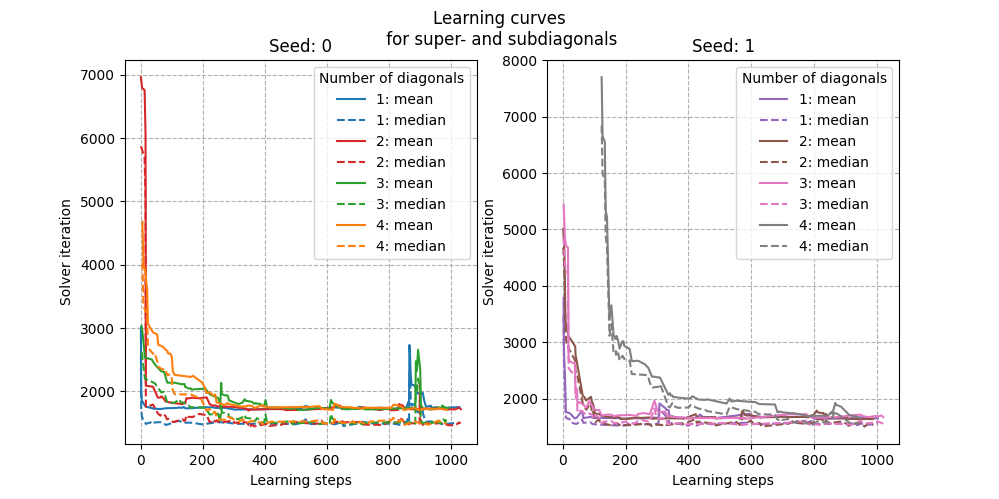
\includegraphics[width=1\textwidth]{plots/super_sub_learn_curve.png}
    \caption{Learning curves for the preconditioner that uses both the super and subdiagonal with a plot for each of the two seeds, with colour corresponding to a different number of super- and subdiagonals  and linestyle corresponding to mean or median solver iteration count.}
    \label{fig: super sub learning curves}
\end{figure}

In the evaluation of the learned preconditioners there also is a major improvement. The mean and median solve iteration counts is around 400 iterations fewer compared to Jacobi preconditioning for all diagonal counts and both seeds, figure \ref{fig: super sub test measure}. Where the previous preconditioners with only the superdiagonal was on par with jacobi preconditioning. In the individual comparison, figure \ref{fig: super sub BvJ}, there is a similar improvement, because all preconditioners have more than 240 systems with lower iteration count compared to Jacobi preconditioning, with 1 super- and 1 subdiagonal begin best for both seeds.

\begin{figure}[H]
    \center
    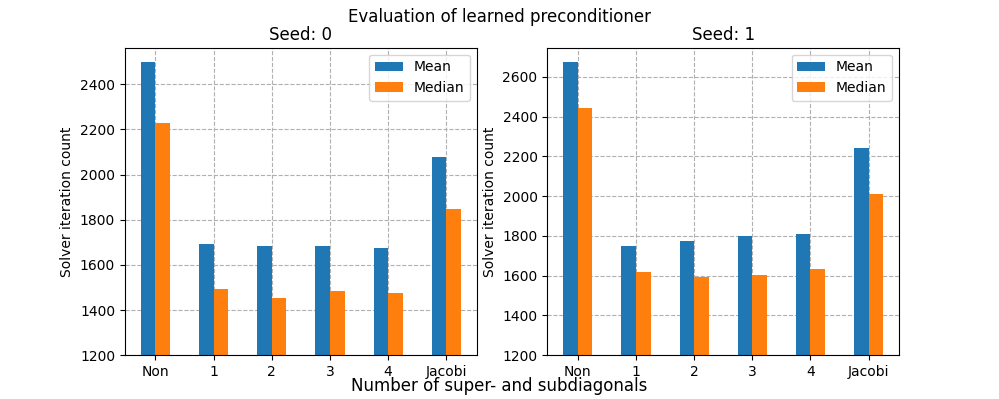
\includegraphics[width=1\textwidth]{plots/super_sub_test_measure.png}
    \caption{Mean and median solver iteration count for the evaluation of the learned preconditioners with different number of super- and subdiagonals, with a plot for each of the two seeds. With colour corresponding to mean or median solver iteration count.}
    \label{fig: super sub test measure}
\end{figure}

\begin{figure}[H]
    \center
    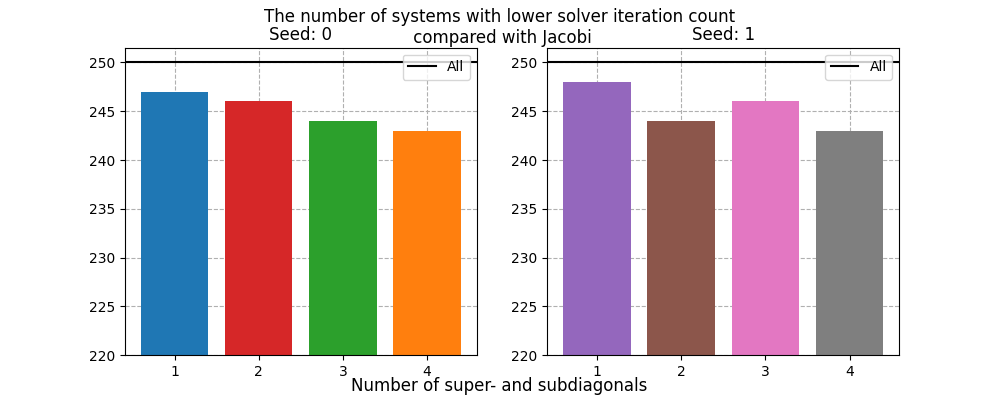
\includegraphics[width=1\textwidth]{plots/super_sub_BvJ.png}
    \caption{Bar graph showing how many individual systems that has a lower solver iteration count with the learned preconditioners compared with its Jacobi preconditioned counterpart, with a plot for each of the two seeds.}
    \label{fig: super sub BvJ}
\end{figure}
